\section{CP Decomposition}
By convention, let $\mathbf{A}\in\RR^{I\times J}$ be a matrix, we shall denote by $\mathbf{a}_j \in \RR^{I}$, where $1\le j \le J$ the $j$-th column of $\mathbf{A}$. Let $\X\in\RR^{I\times J\times K}$ be an order-3 tensor. The CP decomposition seeks for matrices $\mathbf{A}\in\RR^{I\times R}$, $B\in\RR^{J\times R}$ and $C\in\RR^{K\times R}$ such that
\begin{equation}
    \X = \sum\limits_{r=1}^{R} \mathbf{a}_r\circ \mathbf{b}_r \circ \mathbf{c}_r,
\end{equation}
such that $R$ is the smallest possible number. In such case, $R$ is called the \textit{rank} of $\X$. It is usually useful to standardize the column vectors of the matrices to unit norm by introducing scaling factors $\bm{\lambda} = (\lambda_1,\ldots,\lambda_r)^\top$, i.e.
\begin{equation}
    \X = \sum\limits_{r=1}^{R} \lambda_r\,\mathbf{a}_r\circ \mathbf{b}_r \circ \mathbf{c}_r.
\end{equation}

The decomposition can be described briefly as $\X=[[\bm{\lambda}, \mathbf{A}, \mathbf{B}, \mathbf{C}]]$. Let $\Lambda = \mathrm{diag}(\lambda)$, we have the equivalent matricization expressions
\begin{equation}
    \label{eq:matricization}
    \begin{cases}
        \mathbf{X}_{(1)} = \mathbf{A}\Lambda(\mathbf{C}\odot \mathbf{B})^\top \\
        \Xbf_{(2)} = \mathbf{B}\Lambda(\mathbf{C}\odot \mathbf{A})^\top       \\
        \Xbf_{(3)} = \mathbf{C}\Lambda(\mathbf{B}\odot \mathbf{A})^\top.
    \end{cases}
\end{equation}

There is no known finite algorithm for determining the rank of a tensor \cite{kruskal1989rank}. Therefore, for each $R=1,2,\ldots$, we attempt to minimize the difference between $\X$ and a rank-$R$ tensor $\hat{\X}=[[\bm{\lambda}, \mathbf{A}, \mathbf{B}, \mathbf{C}]]$, i.e.
\begin{equation}
    \min\limits_{\hat{\X}}\|\X-\hat{\X}\|^2
\end{equation}

until the difference is less than a given tolerance. Using (\ref{eq:matricization}), we can write, for example, mode-$1$ matricization form of the problem as
\begin{equation}
    \min\limits_{\hat{\X}}\|\X_{(1)} - \mathbf{A}\Lambda(\mathbf{C}\odot \mathbf{B})\|.
\end{equation}

The solution is
\begin{equation}
    \mathbf{A}\Lambda = \X_{(1)}[(\mathbf{C}\odot \mathbf{B})^\top]^\dag = \X_{(1)}(\mathbf{C}\odot \mathbf{B})(\mathbf{C}^\top \mathbf{C}\star \mathbf{B}^\top\mathbf{B})^\dag
\end{equation}

We use the last expression because it requires calculating the pseudoinverse of an $R\times R$ matrix rather than a $JK\times R$ matrix. Therefore, we can solve for each factor iteratively until a convergence criterion is met, particularly, the difference between the original tensor and the reconstructed tensor. The general case for $N$-way tensor is represented in the algorithm below.

\begin{algorithm}
    \caption{CP Decomposition using Alternative Least Square}
    \label{alg:cap}
    \begin{algorithmic}
        \Require $\X\in\RR^{I_1,\ldots, I_N}$, $\epsilon = 1e-10$, $\text{maxIter} = 5000$
        \State Initialize $\mathbf{A}_{(n)}\in\RR^{I_n\times R}$ for $n=1,\ldots, N$ randomly
        \State $\bm{\lambda} \gets \mathbf{0}_R$

        \State $\text{iter} \gets 0$

        \While{$\|\X - [[\bm{\lambda}, \mathbf{A}_{(1)},\ldots, \mathbf{A}_{(n)}]]\|> \epsilon$  and $\mathrm{iter} < \mathrm{maxIter}$}

        \For {$n= 1,\ldots, N$}
        \State $\mathbf{V}\gets \mathbf{A}_{(1)}^\top \mathbf{A}_{(1)} \star \ldots \star \mathbf{A}_{(n-1)}^\top \mathbf{A}_{(n-1)} \star \mathbf{A}_{(n+1)}^\top \mathbf{A}_{(n+1)}\star\ldots\star \mathbf{A}_{(N)}^\top \mathbf{A}_{(N)}$
        \State $\mathbf{A}_{(n)} \gets \Xbf_{(n)} (\mathbf{A}_{(N)}\odot\ldots\odot \mathbf{A}_{(n+1)}\mathbf{A}_{(n-1)} \odot\ldots\odot \mathbf{A}_{(1)})\mathbf{V}^\dag$
        \State $\bm{\lambda} \gets (\mathbf{a}_{(n)1}, \dots, \mathbf{a}_{(n)r})^\top$
        \State Normalize columns of $\mathbf{A}_{(N)}$
        \EndFor

        \EndWhile
        \Ensure $\bm{\lambda}, \mathbf{A}_{(1)},\ldots,\mathbf{A}_{(N)}$.
    \end{algorithmic}
\end{algorithm}

\section{Tucker Decompositions: HOSVD and HOOI}
Let $R_n=\rank(\Xbf_{(n)})$. Tucker decomposition of ranks $S_1,\ldots,S_N$, where $S_n\le R_n$ seeks a tensor $\G\in\RR^{S_1\times\ldots\times S_N}$ and matrices $\Abf_{(n)}\in\RR^{I_n \times S_n}$, where $n=1,\ldots, N$ to minimize

\begin{equation}
    \|\X - \G\times_1\Abf_{(1)}\ldots \times_N \Abf_{(N)}\|.
\end{equation}

The decomposition is written briefly as
\begin{equation}
    \X \approx [[\G, \mathbf{A}_{(1)},\ldots, \mathbf{A}_{(n)}]].
\end{equation}

If $S_n = R_n$, for all $n = 1,\ldots,N$, we have an exact such decomposition, called the higher-order SVD of $\X$ (HOSVD).


\begin{algorithm}
    \caption{Higher-order SVD}
    \begin{algorithmic}
        \Require $\X\in\RR^{I_1,\ldots, I_N}$

        \For {$n = 1,\ldots, N$}
        \State $\Abf_{(n)} \gets R_n$ leading left singular vectors of $\Xbf_({n})$
        \EndFor

        $\G = \X\times_1\Abf_{(1)}^\top\ldots \times_N \Abf_{(N)}^\top$

        \Ensure $\G, \mathbf{A}_{(1)},\ldots,\mathbf{A}_{(N)}$.
    \end{algorithmic}
\end{algorithm}

In the case there exists $S_n < R_n$ for some $n = 1,\ldots, N$, taking $S_n$ left singular vectors of $\Xbf_{(n)}$ as in HOSVD does not lead to an optimal solution. We use the Higher-order Orthogonal Iteration (HOOI) approach with HOSVD as an initialization.

\begin{algorithm}
    \caption{Higher-order Orthogonal Iteration}
    \begin{algorithmic}
        \Require $\X\in\RR^{I_1,\ldots, I_N}$, $\epsilon = 1e-10$, $\text{maxIter} = 5000$.
        \State Initialize $\mathbf{A}_{(n)}, n=1,\ldots, N$ using HOSVD.

        \While{$\|\X - [[\G, \mathbf{A}_{(1)},\ldots, \mathbf{A}_{(n)}]]\|> \epsilon$  and $\mathrm{iter} < \mathrm{maxIter}$}
        \For {$n = 1,\ldots, N$}
        \State $\Y \gets \X \times_1 \Abf_{(1)}^\top \ldots \times_{n-1} \Abf_{(n-1)}^\top  \times_{n+1} \Abf_{(n+1)}^\top \ldots \times_N \Abf_{(N)}^\top$
        \State $\mathbf{A}_{(n)} \gets S_n$ singular vectors of $\Ybf_{(n)}$
        \EndFor
        \EndWhile

        $\G = \X\times_1\Abf_{(1)}^\top\ldots \times_N \Abf_{(N)}^\top$

        \Ensure $\G, \mathbf{A}_{(1)},\ldots,\mathbf{A}_{(N)}$.
    \end{algorithmic}
\end{algorithm}


\section{Implementation Details}

Implementation is organized into three main classes: Tensor, Tensor Builder and Matrix Product. Dependencies are shown in Figure \ref{fig:dependencies}.

\begin{figure}
    \centering
    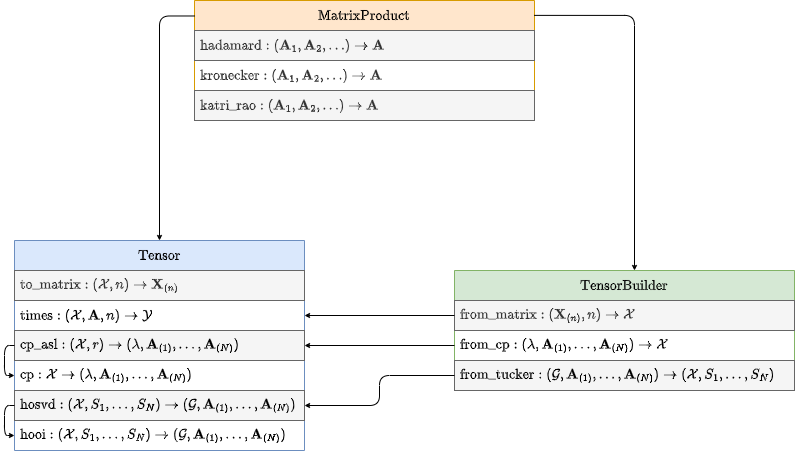
\includegraphics[width=0.8\textwidth]{img/dependency.png}
    \caption{Dependencies between classes and methods}
    \label{fig:dependencies}
\end{figure}

Testcases can be found in \texttt{testcase\_generator.m}, including analytically solvable $2\times2\times2$ tensors to check validity and convergence. Random tensors are also used to check convergence.

\begin{figure}
    \centering
    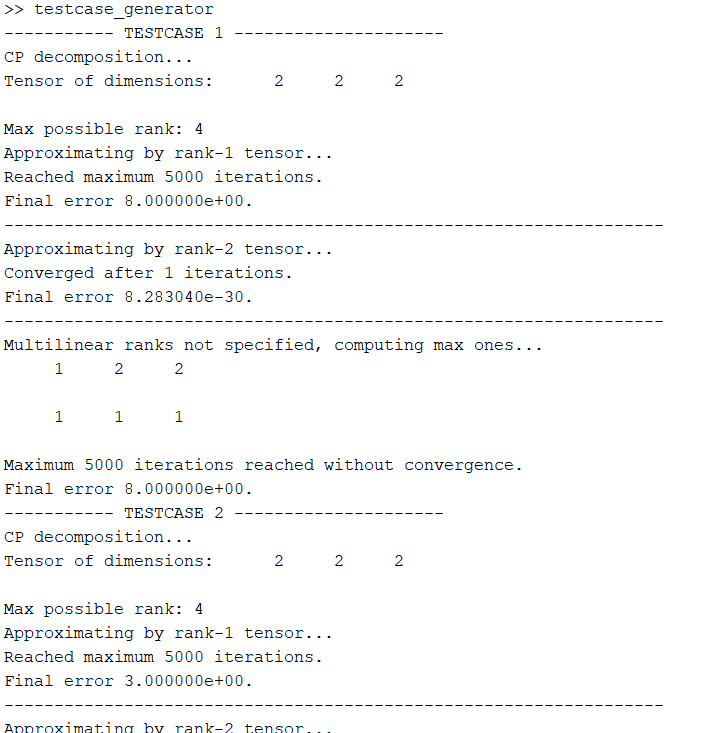
\includegraphics[width=0.8\textwidth]{img/testcases.png}
    \caption{Test run result}
    \label{fig:test}
\end{figure}
